\chapter{Diseño}

El robot Scorbot cuenta con una unidad de control propietaria que permite movimiento por ejes y cartesiano a través de un \textit{teach pendant}. También puede ser conectado a un ordenador mediante puerto serial, para el envía de posiciones y trayectorias predefinidas. Lamentablemente el software de control ha quedado obsoleto, pues solo era compatible con MS-DOS, limitando el uso del dispositivo.

Esta limitaciones abren la puerta para el desarrollo de un hardware y software de control del robot, esta vez de basado en herramientas de código libre y estándares industriales que garanticen una mayor vigencia. Además, hacer que el hardware y software del robot sean compatibles con \textit{frameworks} de robótica, reduce el tiempo y dificultad en tareas de integración y creación de nuevas aplicaciones, mejorando su posibilidad de uso futuro.

\section{Controladores} \label{cap3_controladores}

La función principal de los controladores es el manejo del movimiento de un motor DC. Para realizar esta tarea el controlador debe contar con un microcontrolador, encargado de realizar las tareas de computo y comunicación, y una etapa de potencia, quien transfiere al motor los comandos.

Se consideró que los nuevos controladores fueran capaces de, al menos, tener el mismo desempeño que los originales, de esta forma se establecen una serie de requerimientos:

\begin{itemize}
\item El control distribuido, cada uno de las articulaciones del robot será controlada de forma independiente por un un controlador.
\item Sistema de comunicación capaz de soportar una frecuencia de actualización de 1 \si{\kilo\hertz}.
\item Microcontrolador capaz de establecer un control de corriente a una frecuencia de 10 \si{\kilo\hertz}.
\item La etapa de potencia debe ser capaz de controlar motores DC de 12 \si{\volt} con un consumo \textit{peak} de 8 \si{\ampere}. La frecuencia de conmutación debe ser al menos de 20 \si{\kilo\hertz}, para reducir el rizado de corriente y quede fuera del rango audible. 
\end{itemize}

\subsection{Microcontrolador}

El microcontrolador escogido corresponde al XMC4800 de Infineon Technologies AG, corresponde a un microcontrolador con núcleo ARM Cortex M4 con unidad de punto flotante, incorpora una serie de perifericos útiles utiles para el desarrollo de sistema de control, múltiples \textit{timers} para generación de PWM, interfaz para lectura de encoders (POSIF) y módulo comunicación EtherCAT integrado. La Figura \ref{cap3_xmc4800_data} muestra los distintos módulos que posee el XMC4800.

\begin{figure}[ht]
  \centering
  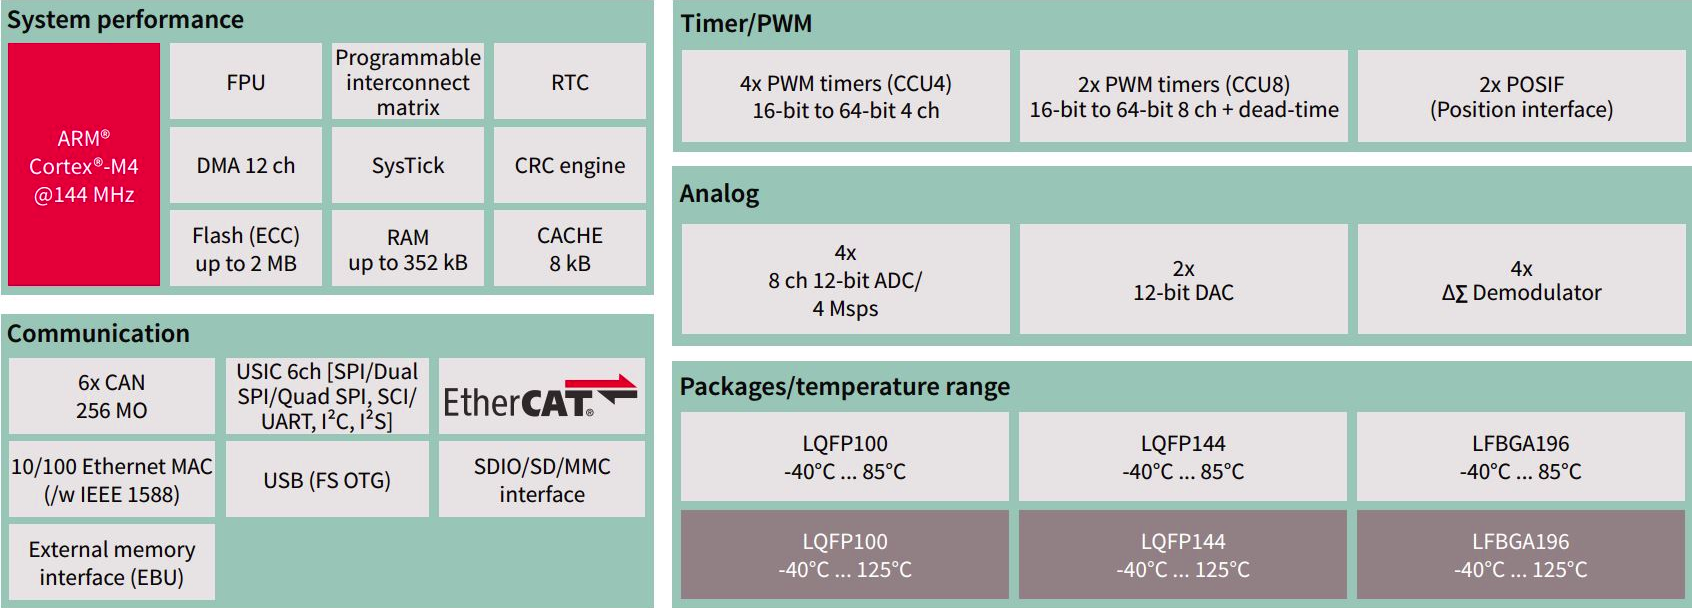
\includegraphics[scale=.2]{img/cap3/xmc4800_data}
  \caption{Carácteristicas del microcontrolador XMC4800. MO: Message Objects, Msps: Mega samples per second.}
  \label{cap3_xmc4800_data}
\end{figure}

\subsection{Puente H}

Funciones especificas

\section{Integración de hardware}

Esquematico y componentes

\subsubsection{PCB}

Placa PCB

\section{Bus de campo}

Conexión

\subsection{Uso de librerías de Ethercat}

SOEM
Flanders Mechatronics Technology Centre has decided to release their EtherCAT PR2
Ig gmbh

